\documentclass[10pt]{beamer}

\usetheme[progressbar=frametitle]{metropolis}
\usepackage{appendixnumberbeamer}

\usepackage{booktabs}
\usepackage[scale=2]{ccicons}

\usepackage{pgfplots}
\usepgfplotslibrary{dateplot}

\usepackage{xspace}
\newcommand{\themename}{\textbf{\textsc{metropolis}}\xspace}

\usepackage[normalem]{ulem}

\usepackage[utf8]{inputenc}
\usepackage[T1]{fontenc}

\title{Parity violation in atomic and molecular physics}
\author{Pierre Bataille and David Rey under the supervision of Benoît Darquié}
\date{February 6, 2018}
\institute{M2 LuMI 2017-2018}


\begin{document}

\maketitle

\begin{frame}{Table of contents}
  \setbeamertemplate{section in toc}[sections numbered]
  \tableofcontents[hideallsubsections]
\end{frame}

\section{Introduction}

% L'énoncé du théorème est à revoir, il y a des phrases qui me semblent douteuses...
% Faire un schéma pour chacun des items de la liste, ce sera beaucoup plus clair.

\begin{frame}{Noether's theorem}

	\begin{itemize}

		\item<2-> Conservation of energy $\Leftrightarrow$ Invariance with respect to time
		\item<3-> Conservation of momentum $\Leftrightarrow$ Invariance by translation
		\item<4-> Conservation of angular momentum $\Leftrightarrow$ Invariance by rotation
		\item<5-> Conservation of parity (P) $\Leftrightarrow$ Symmetry of reflexion
		\item<6-> Conservation of charge conjugaison (C) $\Leftrightarrow$ Change from particle to antiparticle
		\item<7-> Conservation by time reversal (T) $\Leftrightarrow$ Change of the time t by -t

	\end{itemize}

\end{frame}


\section{The weak interaction: the interaction which violates parity}

\begin{frame}{Parity non-conservation}

	% Mettre une figure qui illustre ce que sont la conservation et la non-conservation de la parité.
	
\end{frame}

\subsection{The $\theta-\tau$ puzzle}

% Mettre les décompositions qui font apparaître theta et tau (ça existe?) ainsi que les procédés de décomposition. Ou les valeurs de la masse, quelque chose de visuel pour bien montrer à la fois leurs similitudes et leurs différences.

\begin{frame}{Parity violation in the $\beta$-decay of the cobalt 60}

	\begin{equation}
		Co^{60} \rightarrow Ni^{60} + e^{-} + \nu + \bar{\nu}
	\end{equation}

	\begin{figure}[h!]
		\centering
		\makebox[\textwidth][c]{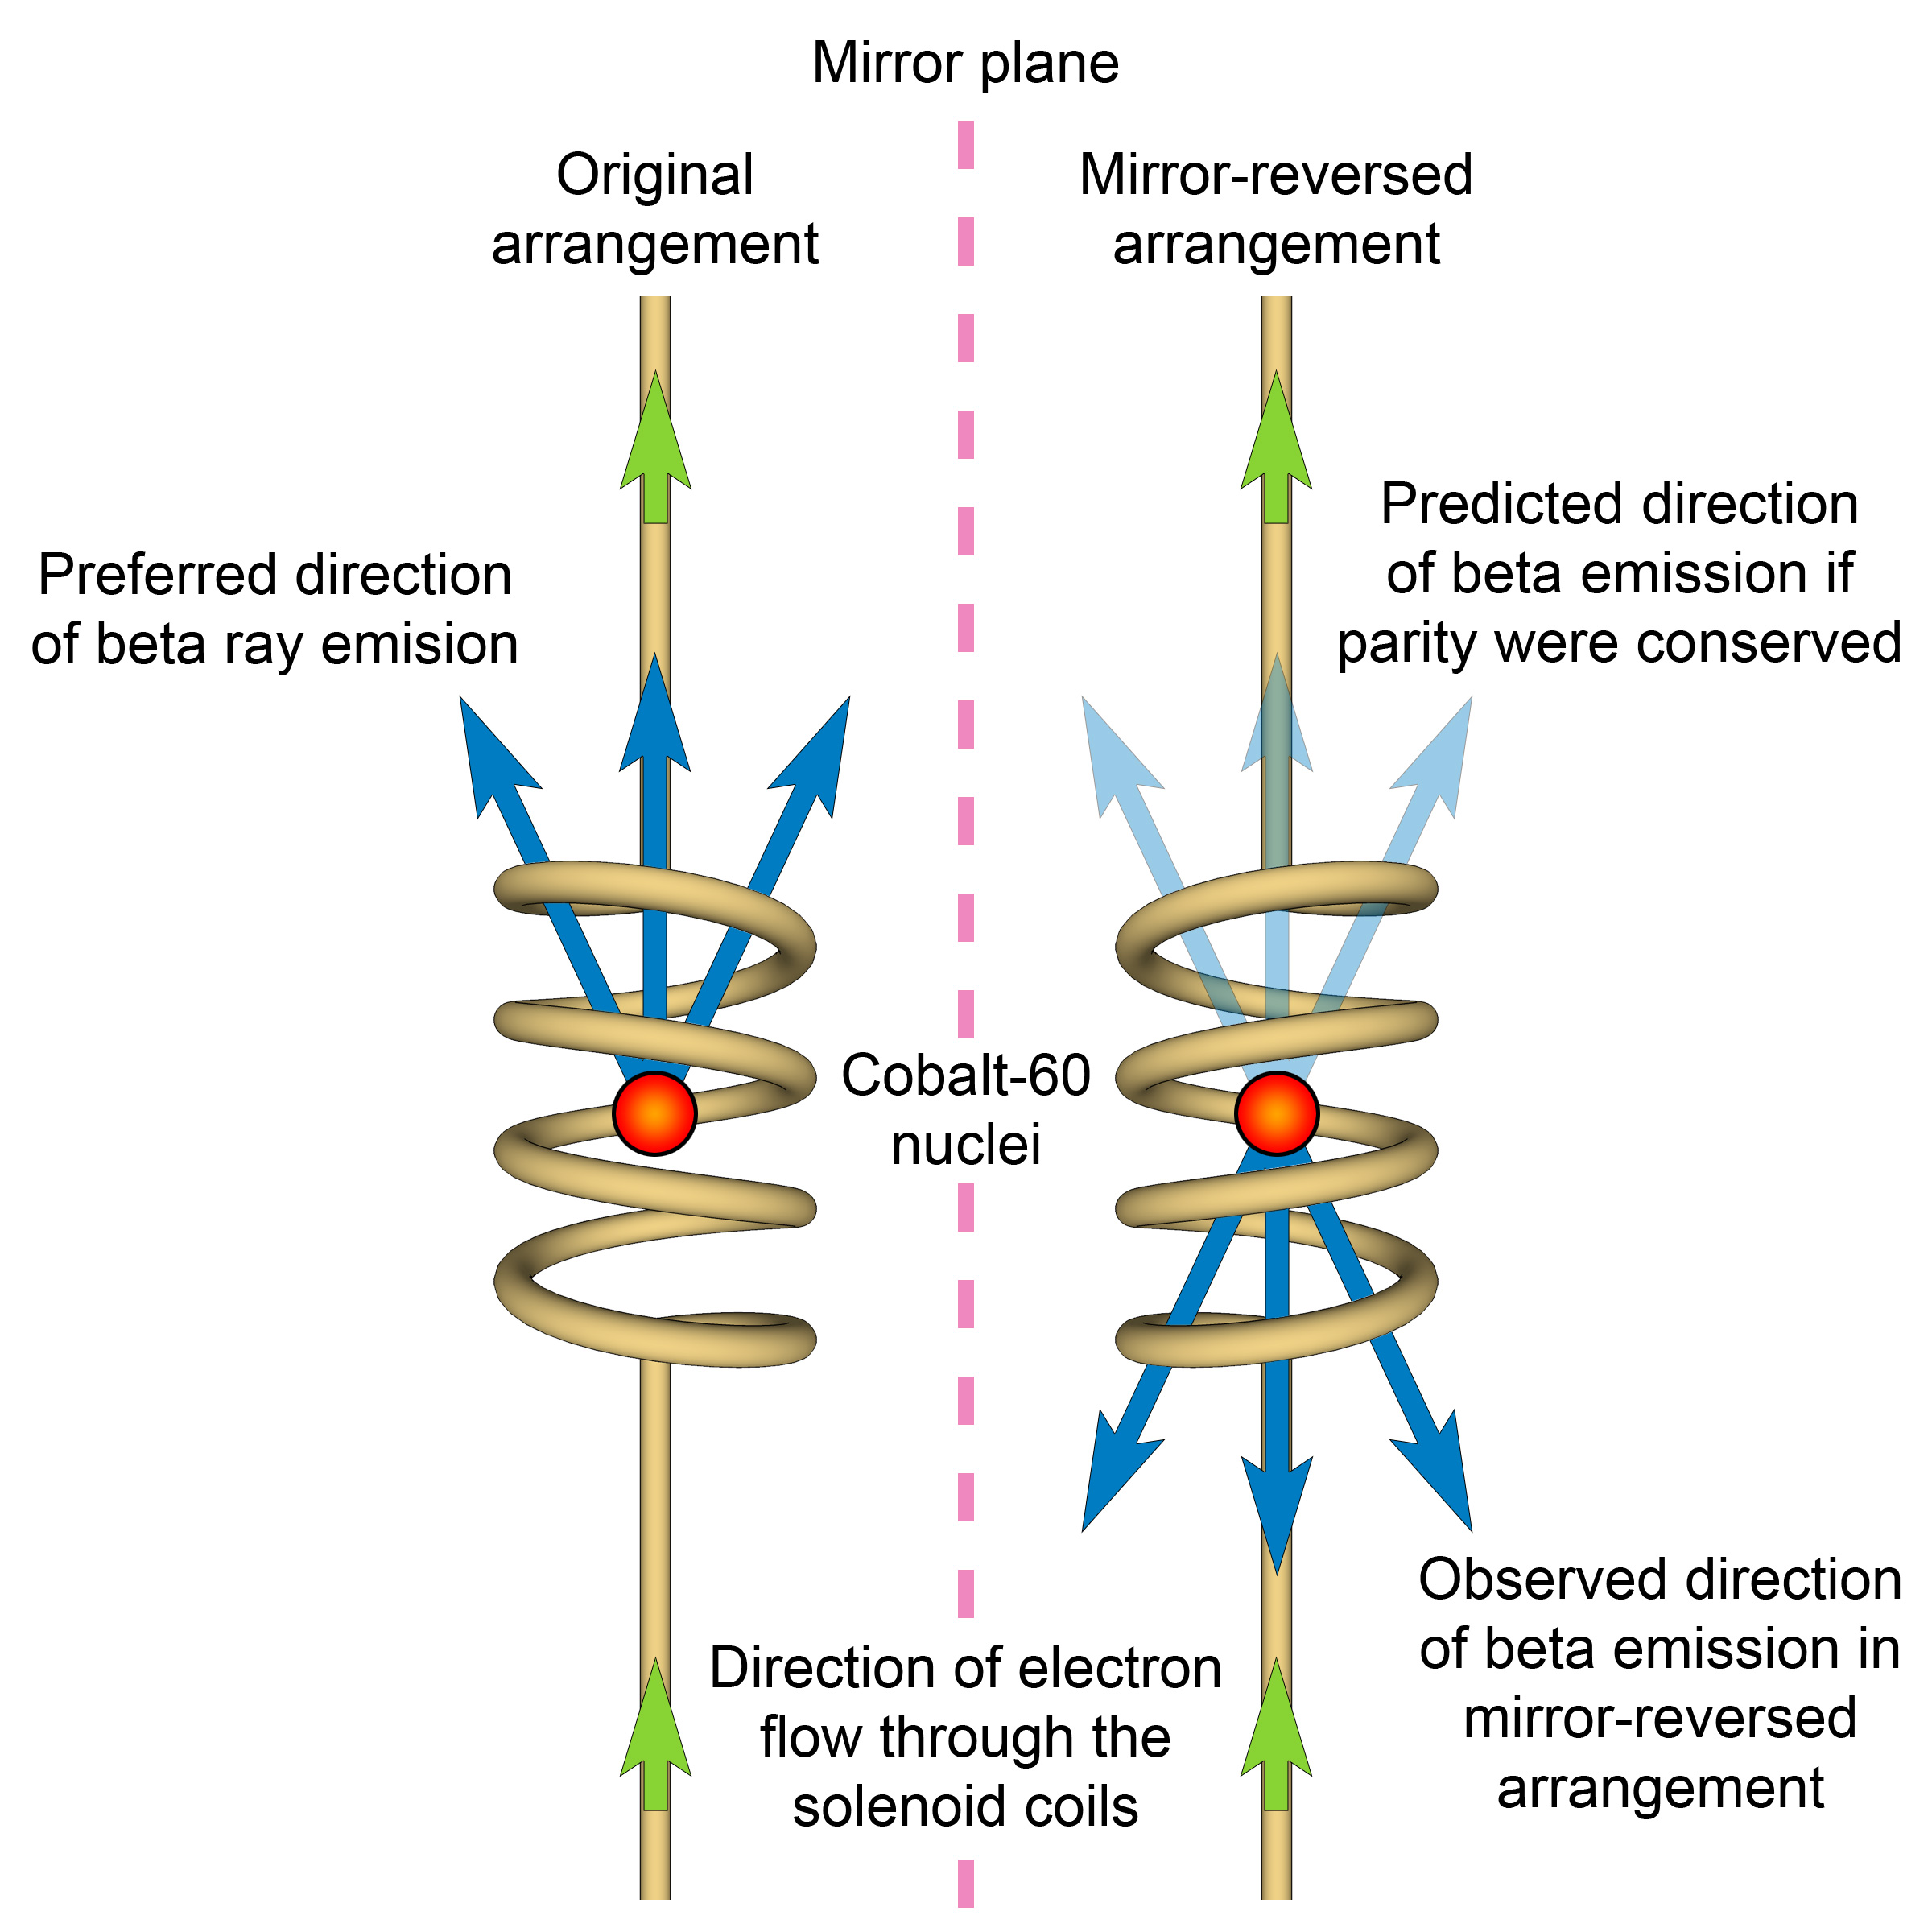
\includegraphics[width=0.6\textwidth]{wu_experiment.jpg}}
		\caption{C. S. Wu experiment.}
		\label{fig:wu}
	\end{figure}

\end{frame}

\begin{frame}{Intermediate vector bosons}

	\begin{itemize}

		\item $W^{+}$: charge $+\textit{e}$
		\item $W^{-}$: charge $-\textit{e}$
		\item $Z^{0}$: neutral particle 

	\end{itemize}

We will focus on \textbf{neutral current weak interactions}, mediated by $Z^{0}$.

% Préciser ce que sont les "neutral current weak interactions" et pourquoi elles nous intéressent dans le contexte de la violation de la parité atomique.

\end{frame}

\section{Measuring parity non-conservation in neutral atoms}

\begin{frame}{Optical activity of an atomic gas}

	% Insérer l'image de Bouchiat (ou autre) pour montrer ce qu'est l'activité optique et montrer comment on peut symétriser une expérience en changeant le champ.

\end{frame}

\begin{frame}{The $Z^3$ law}

	PNC stems from:
	\begin{itemize}

		\item<1-> the coupling between nucleons and electrons\only<4->{ $\propto Z^3$}
		\item<2->\only<2>{the coupling between electrons}\only<3->{\sout{the coupling between electrons}}

	\end{itemize}

\end{frame}

\begin{frame}{The anapole moment}

	\begin{figure}[h!]
		\centering
		\makebox[\textwidth][c]{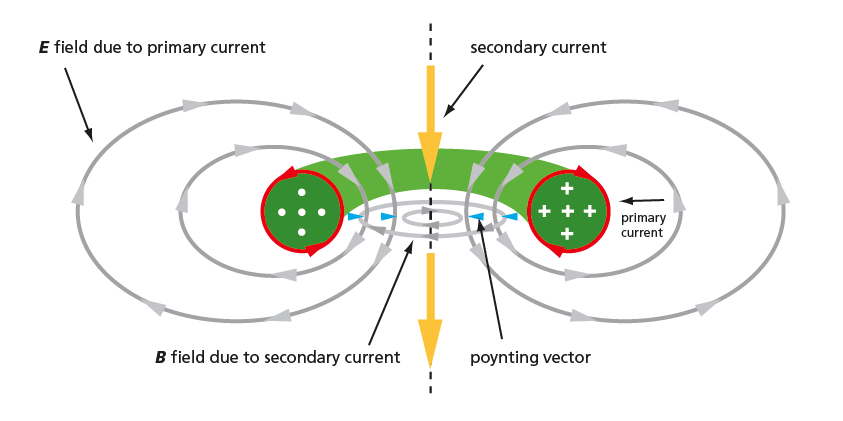
\includegraphics[width=1\textwidth]{b_1_q_0_p_0.jpg}}
		\caption{The fields generated by the current around a toroid}
		\label{fig:AnapoleMoment}
	\end{figure}

	% Il faut fouiller ce truc un peu mieux... Idéalement, il faudrait expliquer les processus internes qui font que c'est bien la manifestation d'une violation de la parité. C'est important pour la compréhension de l'importance de la manip de césium, je pense, bien qu'on peut envisager de la présenter en disant qu'on retourne les champs et que donc toute différence entre deux configurations du champ, c'est de la violation de la parité. 

\end{frame}

\section{Motivations}

\begin{frame}{Explaining biological homochirality}

	% Préciser que ce sont les acides aminés, et peut-être essayer de trouver la représentation de Cram d'un acide aminé simple à représenter, et barrer sa forme R et pas sa forme S.

	% Penser à nuancer le propos en rappelant ce que disait Darquié sur les autres explications possibles.

\end{frame}


\begin{frame}{Testing the standard model}
	
	% Ici, donner des ordres de grandeur : Quelle précision faudrait-il atteindre pour pouvoir tester le modèle standard? Essayer d'éclaircir dans quelle mesure la violation de la parité peut aller à l'encontre du standard model ou au contraire nous permettre de mieux comprendre certaines choses.

\end{frame}


\section{Measurement of parity non-conservation and an anapole moment in cesium}

\begin{frame}
	
	% Mettre la classification périodique des élements en entourant le césium, pour montrer pourqoi c'est une espèce intéressante : calculs faciles mais Z grand.

	\begin{figure}[h!]
		\centering
		\makebox[\textwidth][c]{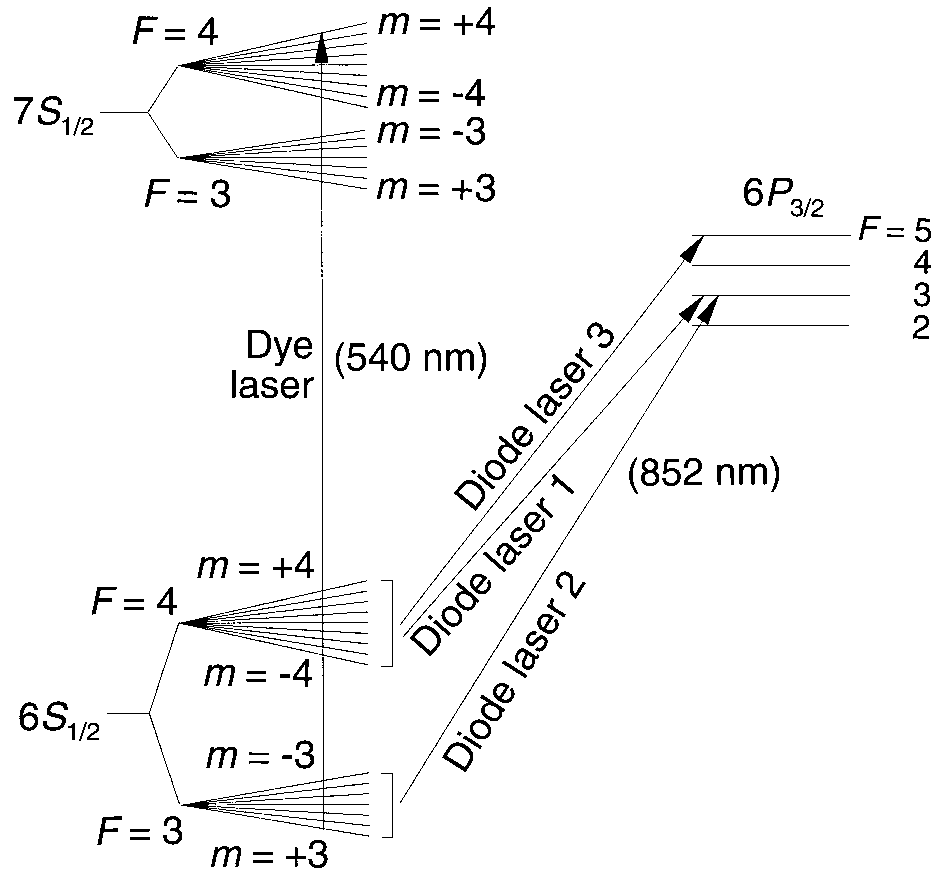
\includegraphics[width=0.8\textwidth]{cesium_states.png}}
		\caption{The energy level diagram of cesium}
		\label{fig:cs}
	\end{figure}

	

\end{frame}

\begin{frame}{Principle}

	

\end{frame}

\begin{frame}{Experiment}

	

\end{frame}

\end{document}
